\documentclass{article}
\usepackage[utf8]{inputenc}

\usepackage{indentfirst}
\usepackage{url}
\usepackage{hyperref}
\usepackage{graphicx}
    \DeclareGraphicsExtensions{.png, .jpg, .jpeg}
    
\usepackage{biblatex}
\addbibresource{P2_Team_02.bib}

\title{CS791 Project 2: Experimental Setup \\ A Usability Evaluation of a Public Collaborative Data Portal}
\author{\emph{Team 2}: Terence Henriod, Vinh Le \\ \emph{Instructor}: Sergiu Dascalu}
\date{\today}

\begin{document}

% Title Page Needs:
% university
% department
% course
% project title
% project part
% team number
% authors
% instructor
% date

\clearpage            % necessary for removing page number on first page

\maketitle
\begin{center}

\includegraphics[scale=0.4]{unr-logo} \\[0.5cm]
\textsc{\Large University of Nevada, Reno} \\[0.5cm]
\textsc{\large Computer Science and Engineering Department} \\
\end{center}

\thispagestyle{empty} % removes the page number from the title page

% create some whitespace between title stuff and abstract
\vspace{10mm}

%
%
\newpage
\section{Introduction}
The NRDC grown exponentially over the past two years; its initial user base started with a select few individuals and has grown to accommodate almost three thousand users. New services are added routinely as the system encompasses more and more projects. As development continues for the NRDC, it is vital that the current services are continually optimized for a better user end experience or else risk a loss of attraction in the eyes of its users. The idea of this project is to perform a user study on the main services present within the system in order to extrapolate a plausible future direction for the NRDC. In this user study, participants will be utilizing the already developed web services located on the NRDC, whilst providing feedback based on ease of usage. 

One of the main ideals that make up Human and Computer Interaction (HCI) is the pursuit or development of a better user end experience. As this study is designed to find that better experience, this project holds a great deal of relevancy to the field of HCI. The NRDC is heavily affiliated with the Department of Computer Science and Engineering (CSE), which allows for an easier access to references and support, thus making the choice of having this user study very attractive. Additionally, this study would benefit the members of the CSE department, as well as the National Science Foundation, making this a fantastic choice to give back to the both organizations, as we have been affiliated with them in the past.

In the end the final goal of this user study is to developed a more intuitive system, which balances pragmatism and a user friendly approach, for the services in the Nevada Research Data Center.

%
%
\section{Methodology}
%
\subsection{Participants}
In this user study, we will gather at least 6 participants, all of whom will be students or researchers from the University of Nevada, Reno. The NRDC aims to provide data services to students and researchers aiming to complete research in the state of Nevada. In light of this, each of these participants will be members of a mainly research-oriented major, such as Computer Science and Engineering, Math, and Physics, in order to simulate a likely situation of usage as possible. These participants will have never touched the system before and minimal training will be issued in order to close any gap of skill in between participants (it is recommended that uninitiated users are actually good candidates for exposing usability difficulties\cite{dontmakemethink}). Participants will be recruited through affiliated graduate organizations, local philanthropy events, and various student organizations on campus. The experiment itself will be brief and refreshments will be offered as suitable compensation.

%
\subsection{Apparatus}
\subsubsection{NRDC}
The NRDC is the web interface itself that is the target of evaluation for this user study. The NRDC is a web portal containing various services that are linked on the main page of the NRDC itself. Both versions of the NRDC will be used, the version currently in deployment and the new one currently in development. The web services on the NRDC are: the WebCam Image Archive, the Geospacial Data Search, and Current Conditions. The WebCam Image Archive is a service that allows users to navigate to all of the current research sites affiliated with the NRDC. Users will have the ability to save, view, and download webcam images taken during a specified time each day. Additionally, users may also have these images stringed together to form a video with the option of downloading it. The Geo-spatial Data Search allows users to navigate to an affiliated research site through Google Maps and retrieve actual quantifiable data by narrowing down the the filter and dates. The Current Conditions provides users with the ability of retrieving live research data at a specified research site through Google Maps.

\subsubsection{Work Station}
Users will use a typical Windows desktop workstation with a standard monitor, keyboard, and mouse. The workstation will be in a typical group office/workspace (the Cyber Infrastructure Lab, located in the Scrugham Engineering and Mines building, room 255, at the University of Nevada, Reno), which should afford participants a relatively calm working environment. This standard setup should be very comparable to the typical workspace used by typical NRDC users.

\subsubsection{Tasks and Data Collection}
To present tasks and collect timings, a third-party mobile phone application, named \emph{HCI-Task}, will be used. This will be a simple Android application used on a 4+" touchscreen smart phone that will allow users to swipe between a text description of the task and a screen shot of the goal state for the task, as well as declare when a task has been completed or given up on.

%
\subsection{Procedure}
The steps of the experiment will be conducted for each user as follows:
\begin{enumerate}
\item Participant will be greeted, and then given a brief description of what the NRDC, its purpose, and what the reason for conducting a user study is.

\item Participants will be directed to a workstation and briefly shown how to access the NRDC interface version they have been assigned to work with (which will be labeled in such a way as to not introduce bias as labels like "new" and "old" might).

\item Participants will be given the smart phone that will display the tasks that they are to complete, introduced to the NRDC interface they will be starting with, and walked through an initial training task. This will help mitigate the effects of participants being too unfamiliar with what the goals of the study are to be effective.

\item Participants will then complete 2 more tasks on their own, as quickly as possible. The phone will display the task prompts and collect performance data. Users will be allowed to give up on tasks after 4 minutes if they feel frustrated or discouraged.

\item A short break will be taken. The researchers will prepare for the next step, and possibly have casual conversation with the participant.

\item Participants will again be directed to complete another task as quickly as possible, this time with the other NRDC interface.

\item Participants will complete a survey composed of both Likert scale and open-ended questions regarding their subjective assessment, preferences, and suggestions about the NRDC and its interfaces.

\item Finally, participants will be debriefed, allowed to ask questions, and offered refreshments as compensation for their participation.
%
\end{enumerate}

% For the user study, participants will be scheduled one after another with a rest period of about five minutes between each. The experiment itself will consist of a two major phases. The first phase will include a training phase where the participants are given a brief overview of tasks and tasked with a sample query of data on a common web portal in order to mitigate any experience gaps in participants. The second phase will begin the testing of the services where each participant is given a set of seemingly brief tasks to be completed in the shortest time possible. Each participant will be asked to retrieve varying sorts of data from every service and must return to the original service interface and eventually the portal itself before concluding. Half of the participants will be given the current interface while the other group will use the new interface. At the end of the entire experiment, participants will be given time to complete their questionnaire/feedback form before finally finishing. A sample of the questionnaire can be seen below in figure \ref{fig:placeholder}.

%
\subsection{Tasks}
Participants will be asked to retrieve data from each of the major services that compose the NRDC. The tasks will be timed to measure performance, but users will be given the option to "give up" on any task after 4 minutes to help measure search perseverance in tandem with task performance.

% In terms of tasks assigned to the participants, the participants will be asked to retrieve data from each service. For the Geo-spatial Data Search, the participant must properly retrieve a data set from a randomized date during a random set of hours. For the WebCam Image Archive, the participant must retrieve a collection of images and a video from another set of randomized dates and times. For the current conditions, the participant will be given a random research site and must show the most recent data and time-stamped photo from the interface. The tasks themselves will be timed and measured by the amount of minutes taken to complete each task and the entire total time of the session. Additionally, the feedback form will use a Likert scale to indicate preferences in regards to the process of the search, the UI, and the overall difficulty of the tasks.

\begin{enumerate}
\item Geo-Spatial Data Search
The Geo-Spatial Data Search service provides a variety of data from several very specific locations in the Nevada wilderness. Participants will be asked to retrieve a specific set of (applicable) data from a specific location for a random time period in the past. Variables and locations will be determined ahead of time by the researchers, since not all types of data are available for all locations. This task will be considered complete once the participant has viewed the raw data.
    
%% replace "placeholder" with the name of the image file (just the name, not the extension)
%% Put an appropriate caption
%% make sure to put an appropriate label, usually "fig:<image-file-name>" is good
\begin{figure}[h!]
  \centering
  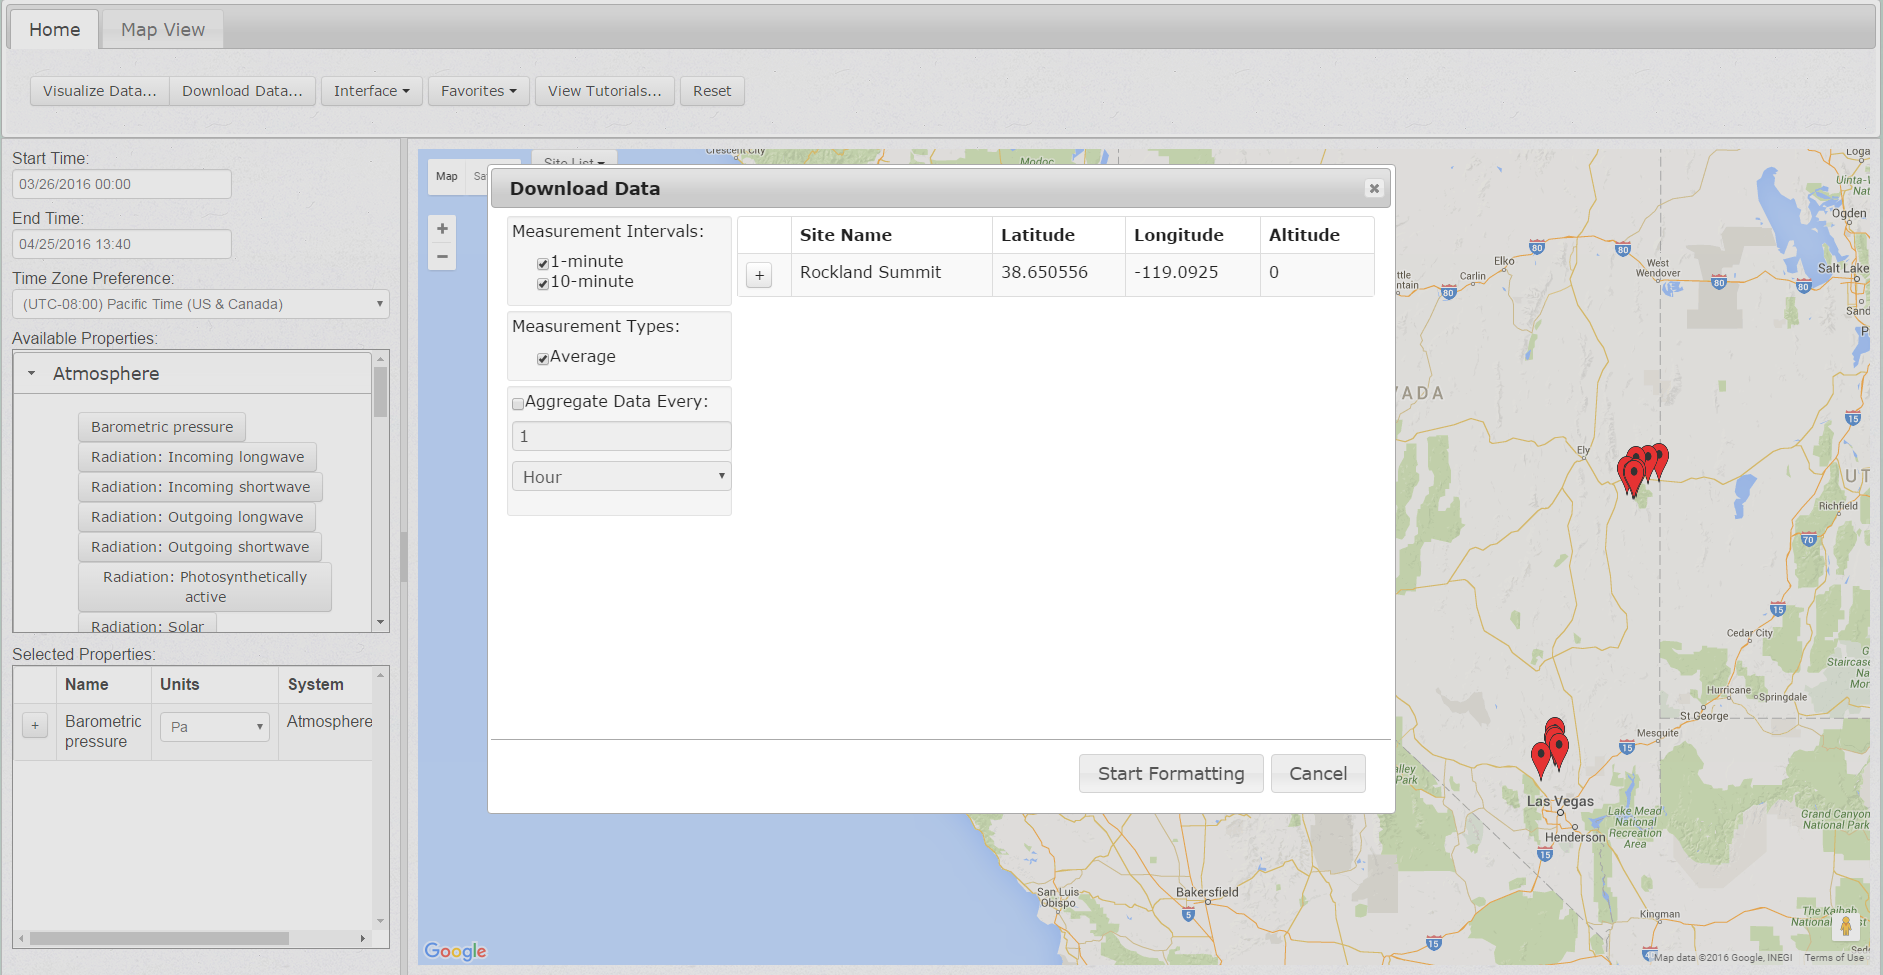
\includegraphics[width=.6\linewidth]{geospatial}
  \caption{A screen shot of some basic data obtained through the Geospatial Data Search.}
  \label{fig:geospatial}
\end{figure}

\item Webcam Image Archive
The Webcam Image Archive features real, sometimes scenic, imagery captured by remote cameras. Participants will be asked to retrieve a collection of images from a particular location and a particular date and time, determined by the researchers beforehand. This task will be considered completed once the participant has been able to scan through the selected image set to verify that it has been retrieved.

\begin{figure}[h!]
  \centering
  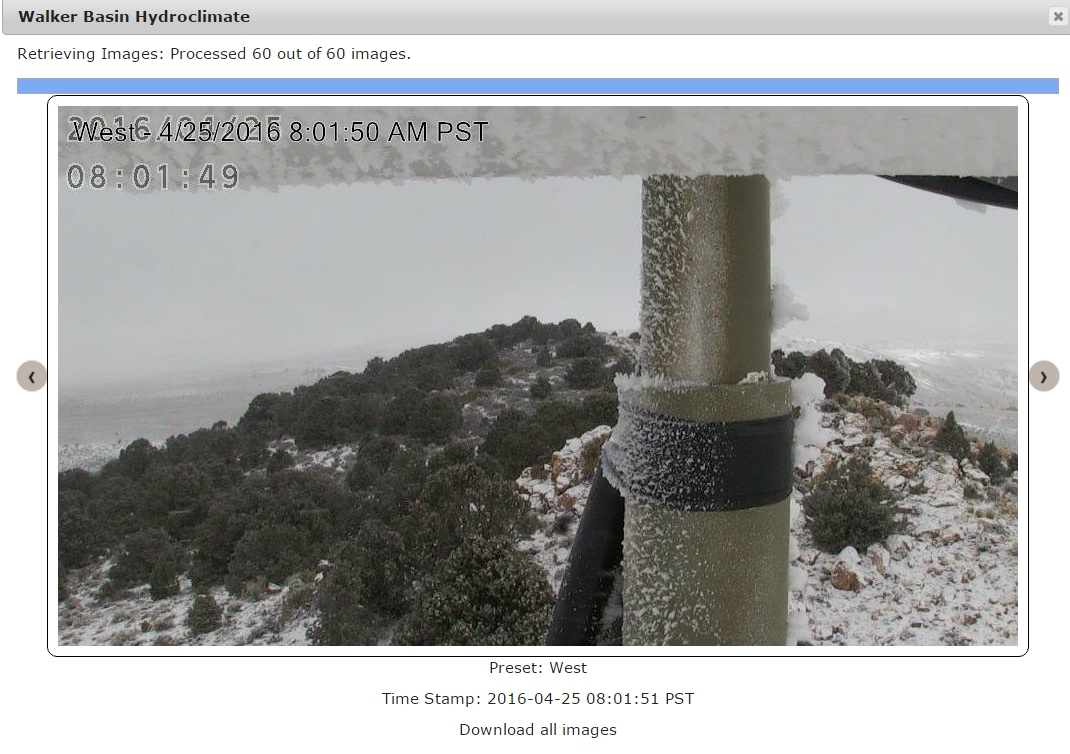
\includegraphics[width=.6\linewidth]{webcam-image-archive-example}
  \caption{A screen shot of the partial results from the a Webcam Image Archive task.}
  \label{fig:webcam-image-archive}
\end{figure}

\item Webcam Streams
The NRDC offers access to remote wilderness cameras that continuously stream live video in various formats. Participants will be asked to locate and view the video stream for a specific location in a specific location, determined beforehand by the researchers. The task is considered complete once participants determine that they are, in fact, viewing a video stream. Participants are not required to view a particular amount of video to prevent the task completion time from being artificially long.

%% replace "placeholder" with the name of the image file (just the name, not the extension)
%% Put an appropriate caption
%% make sure to put an appropriate label, usually "fig:<image-file-name>" is good
% \begin{figure}[h!]
%   \centering
%   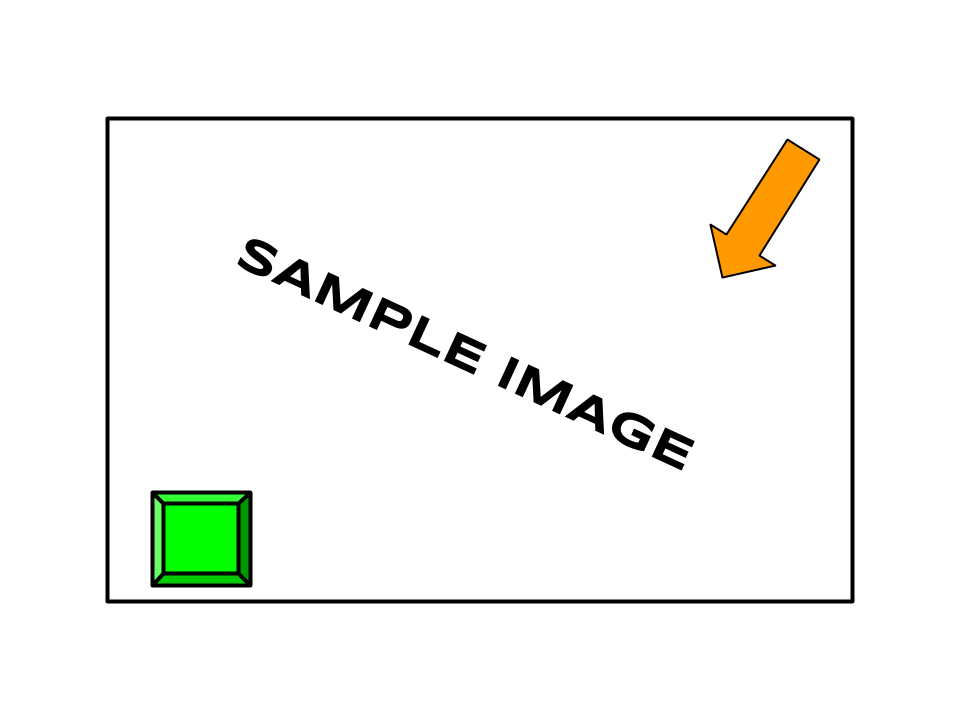
\includegraphics[width=.6\linewidth]{placeholder}
%   \caption{This is a sample image.}
%   \label{fig:placeholder}
% \end{figure}

\item Current Conditions
The Current Conditions service neatly summarizes much of the data for a given location, integrating weather data and a current webcam image. In order to evaluate both the navigability of this feature and the usability of the displayed data, participants will be asked to find the current conditions for a specific location and retrieve the values of two items of the displayed data. The location and which data items will be selected beforehand by the researchers. The task will be considered completed once the participant self-identifies as having found the requested information.

\begin{figure}[h!]
  \centering
  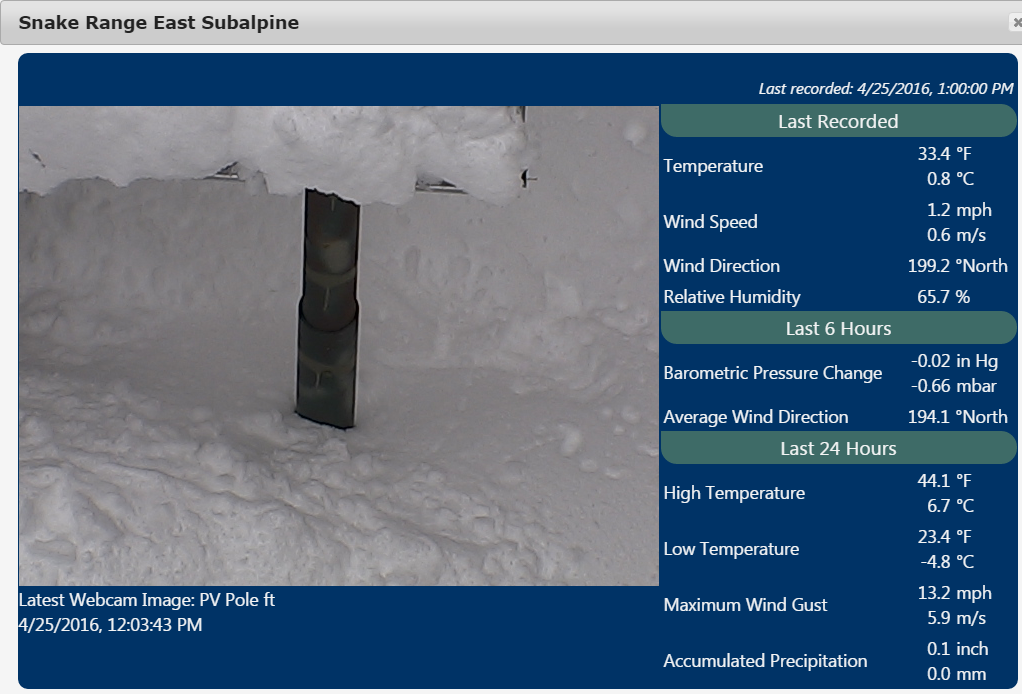
\includegraphics[width=.6\linewidth]{current-conditions-example}
  \caption{An sample screen shot of the Current Conditions interface.}
  \label{fig:current-conditions}
\end{figure}

\item Subjective Analysis
After completing the primary tasks, participants will be asked to rate the NRDC interfaces (current and in-development) in terms of preference, ease of use, and suggestions for improvement. This task is unlike the others in that it is not traditional performance research task per se, nor it it directly related to the NRDC.

%
\end{enumerate}

%
\subsection{Design}
The user study will explore the effect of the version of NRDC interface on task completion performance and subjective response to the interface. The experiment will be a 1 x 2, mixed between- and within-subjects experiment.

The independent variable \emph{Interface Version} will have two levels: \emph{current} and \emph{in-development} (for participants they will be labeled as \emph{Interface 1} and \emph{Interface A} to prevent any biasing inferences). It should be noted that \emph{Interface Version} represents the interface that participants will have their performance measured on, as well as which of the two interfaces participants will encounter first for the subjective evaluation (although, in the second sense, we hope this will have no effect on any of the examined outcomes).

The dependent variable \emph{Task Performance} will be measured in seconds, and the other, \emph{Interface Preference} will be measured using Likert scale responses and collect open-ended feedback. Implicit in \emph{Task Performance} is a thrid dependent variable, \emph{Task Perseverance}, which will simply be a measure of when participants choose to end a task because they feel it is taking unreasonably long to complete. \emph{Task Perseverance} will be a count of how many times a participant "gives up", and will only be analyzed if any concessions are observed.

Control variables will include \emph{Work Setting} (which will be restricted to a small, communal university work space) and \emph{Work Station Type} (which will be restricted to a standard Windows desktop work station).

Due to the two-fold nature of the study, the evaluation of \emph{Task Performance} will be treated as a between-subjects study to eliminate the order-effect of participant learning, but the evaluation of \emph{Interface Preference} will be treated as a within-subjects due to the necessity of participants needing to experience both levels of \emph{Interface Version} to determine a preference.

In order to counterbalance the order-effect of participant preference of one interface or the other, participants will evenly divided between the two levels of \emph{Interface Version}. It is possible that \emph{Interface Version} will be a confounding variable, but we hope to prevent this by giving participants different tasks to complete with their second interface to try and preserve any of the novelty experienced when working with the first interface.

For \emph{Task Performance} measurement, 6 participants x 3 tasks = 18 total tasks will be performed. Overall, however, for the purposes of the \emph{Interface Preference}, 16 participants x 4 tasks = 24 total tasks will be performed.

%
%
\section{Additional Information}
The researchers would like to acknowledge I. Scott MacKenzie\cite{hci-research-perspective} for their excellent text book on conducting empirical research, which guided the design of this experiment; Nakarada-Kordic and Lobb\cite{PerceivedAttractiveness} and Krug\cite{dontmakemethink} for their previous research on web interface usability, and Le, Neff, Stewart, Kelley, Fritzinger, Dascalu, and Harris\cite{microservice-nrdc} for their intial and continued development of the NRDC.

%
%
% \section{About the Authors}
% %
% \subsection{Terence Henriod}

% Terence is a graduate student in the Computer Science and Engineering(CSE) department at the University of Nevada, Reno (UNR). Terence previously graduated with a Bachelor's Degree in Community Health Sciences from UNR and continued his graduate studies in CSE, expecting to finish in May of 2016. Terence has worked in industry for an IoT startup (and maintains a continued interest in IoT), and is excited to begin working at GE Bently in May after graduation.

% %
% \subsection{Vinh Le}

% Vinh is a graduate student in the Computer Science and Engineering department at the University of Nevada, Reno and graduated previously with a Bachelor's Degree in CSE at the very same university. In regards to professional interests, Vinh favors development in software engineering, web technologies, and human-computer interaction.
% 
%
%

\printbibliography

\end{document}
